\documentclass[12pt]{article}
\usepackage{natbib}
\usepackage{hyperref}
\usepackage[french]{babel}
\usepackage[utf8x]{inputenc}
\usepackage{lipsum}
\usepackage{amsmath}
\usepackage{graphicx}
\usepackage[final]{pdfpages}
\usepackage[T1]{fontenc}
%\usepackage[colorinlistoftodos]{todonotes}
\usepackage{xcolor}
\usepackage[nottoc,numbib]{tocbibind}% Para que la bibliografia salga en el table of contents
\colorlet{Mycolor1}{green!10!orange!90!}
\usepackage{subfigure}
\sloppy
\definecolor{lightgray}{gray}{0.5}
\setlength{\parindent}{0pt}
\setlength{\parskip}{1em}

\bibliographystyle{abbrv}

\begin{document}
\title{Rapport Stage}
\author{CHIRINO CAICEDO Melet}
\begin{titlepage}

\newcommand{\HRule}{\rule{\linewidth}{0.5mm}} % Defines a new command for the horizontal lines, change thickness here

\center % Center everything on the page
 
%----------------------------------------------------------------------------------------
%	HEADING SECTIONS
%----------------------------------------------------------------------------------------

\textsc{\LARGE Université Toulouse III}\\[0.5cm] % Name of your university/college
\textsc{\Large Paul Sabatier}\\[1.0cm] % Major heading such as course name
\textsc{\large Rapport du stage 2020/2021}\\[0.5cm] % Minor heading such as course title

%----------------------------------------------------------------------------------------
%	TITLE SECTION
%----------------------------------------------------------------------------------------

\HRule \\[0.4cm]
{ \huge \bfseries Projet Linky4Teens}\\[0.4cm] % Title of your document
\HRule \\[1.5cm]
 
%----------------------------------------------------------------------------------------
%	AUTHOR SECTION
%----------------------------------------------------------------------------------------

% \begin{minipage}{0.4\textwidth}
% \begin{flushleft} \large
% \markboth{Pojet en \LaTeX}
% \emph{Auteurs:}\\
% \textsc{CHIRINO} Melet \\ % Your name
% %\textsc{RIBEIRO} Bruno % Your name
% \end{flushleft}
% \end{minipage}
% ~
% \begin{minipage}{0.5\textwidth}
% \begin{flushright} \large
% \emph{Tuteur:} \\
% \textsc{RIVIERE} Nicolas  \\% Supervisor's Name
% \textsc{LABIT} Yann% Supervisor's Name
% \end{flushright}
% \end{minipage}\\[2cm]

 % If you don't want a supervisor, uncomment the two lines below and remove the section above
\Large \emph{Author:}\\
\textsc{CHIRINO CAICEDO} Melet David \\[2cm] % Your name

%----------------------------------------------------------------------------------------
%	DATE SECTION
%----------------------------------------------------------------------------------------

{\large \today}\\[2cm] % Date, change the \today to a set date if you want to be precise

%----------------------------------------------------------------------------------------
%	LOGO SECTION
%----------------------------------------------------------------------------------------


\includegraphics[width=6in]{img/Logo_UT3.jpg}\\[2cm] % Include a department/university logo - this will require the graphicx package
 
%----------------------------------------------------------------------------------------

\vfill % Fill the rest of the page with whitespace

\end{titlepage}

%\{Contents}
\tableofcontents

\newpage

%-------------------------- * Introduccion * --------------------------------

\section{Introduction}
%Aqui explico de que se trata el proyecto y lo que habiamos hecho antes como TER
Linky4Teens est un projet qui cherche à améliorer la performance des jeunes athlètes avec l'électronique. Ce projet est mené à bien avec le professeur Yann LABIT et le club sportif Balma, image \ref{img:LogoBalma}.
% El proyecto linky4teens es un proyecto que busca desarrollar prototipos que ayuden a mejorar el desempenho en atletas jovenes llevado por el club Balma y el Profesor Yann LABIT. El proyecto busca crear dispositivos para revisar el desempenho de los atletas y trabajar sobre los errores que se esten cometiendo. 

\begin{figure}[!htb]
\centering
\includegraphics[width=0.2\textwidth]{img/LogoBalma.png}
\caption{Club Balma}
\label{img:LogoBalma}
\end{figure}

Ce projet a commencé comme un projet TER dans lequel j'ai travaillé dans le développement d'un témoin intelligent connecté pour la course de relais. En tant que stagiaire, j'ai repris le développement du témoin intelligent connecté et aussi un starting bloc développé par d'autres étudiants pour un projet TER parallèle.
% Yo estaba encargado de seguir el desarrollo de dos prototipos desarrollados en proyectos anteriores como proyectos de TER:
% \begin{itemize}
%     \item Temoin de relevos inteligente (desarrollado por mi un grupo de amigos)
%     \item Starting block
% \end{itemize}
% Estos proyectos al estar financiados por estudiantes estaban bien pero necesitaban mejoras y mucha robustez para funcionar como producto funcional.

%-------------------------- * Descripcion * --------------------------------

\section{Bref description du systeme}
% Aqui vas a mostrar unos cuantos diagramitas UML para explicar como funcionan las cosas dentro tus chocoros
En fin du projet TER le projet avait deux prototypes utilisés pour deux disciplines d'athlétisme différents : Course de relais et un starting bloc.

\begin{itemize}
	\item Le témoin a été conçu pour la course de relais. Le témoin stocke 	des données comme la vitesse horizontal et la  position verticale pour 	savoir des détails lorsqu'ils font le relai.	En plus, le témoin capte aussi si le relais est fait 	dans la zone de relais. Après le témoin est connecté à un 	ordinateur pour voir l'information de la course et faire des 	couvre pour une analyse complète. 

	\item Le starting bloc stocke l'information de deux capteurs de force placés en-dessous des pieds des athlètes pour savoir la force utilisée au debut de la course. Cette information est visible grâce à une curve montrée à travers d'un smartphone.
\end{itemize}

%-------------------------- * Objetivos * --------------------------------

\section{Objectifs}
% Les objectifs pour le debut du projet etaient rendre les prototypes plus robustes pour une utilisation ulterieur.
% Los objetivos de stage eran rendre plus robuste los prototipos ya existentes y/o los sistemas creados.
\begin{itemize}
	\item Améliorer le dock pour rendre plus facile son utilisation car en fin du projet TER était un peu délicat et compliqué à utiliser.
	\item Améliorer l'interface visuelle (GUI en anglais).
	\item Rendre les témoins plus robustes et y stocker plus d'informations.
	\item Rendre plus robuste le prototype du starting bloc et l'intégrer à l'interface déjà développée.
\end{itemize}
\section{Améliorations proposées}
\begin{itemize}
    % \item Dock: utilisar una raspberry pi como dock porque esta puede usar conexion wifi direct a cualquier dispositivo que pueda acceder a internet sin necesidad de instalar porgramas o aplicaciones. 
	\item Utiliser une raspberry pi comme Dock parce 	qu'elle peut se connecter à tous les appareils via Wi-Fi direct pour éviter d'installer l'interface dans tous les ordinateurs du club. En plus, la raspberry peut stocker une base de données avec l'information de tous les coachs et les athlètes.


    % \item Temoin: el temoin estaba soldado en una pcb universal y era muy endeble, habia que volverlo mas robusto y, el punto mas importante, no guardaba suficiente informacion, por lo tanto las mediciones eran medio jopos. Ademas el sistema de barreras IR era poco robusto. Todo eso debia mejorarlo.
	% \item Faire une pcb à l'aide d'un CAO pour ajouter
	% plus de compossants et rendre la partie electronique
	% plus robuste. En plus, ajouter des composants pour 
	% une utilisation plus confortable chez les athletes.
	\item Améliorer le témoin de relais pour capter plus d'informations et pour rendre plus robuste.
    % \item Interfaz: la interfaz utilisaba un deploy de django (un framework web escrito en python porque? porque yo lo se usar, asi de simple). Pero estaba muy simple por propias limitaciones del sistema pero con mas financiacion se podia mejorar todo.
	\item Créer une base de données dans l'interface de tous les acteurs du club Balma pour avoir une traçabilité de la performance des athlètes.
	\item Établir une communication entre le starting bloc et l'interface pour manipuler les données.
	\item Rendre l'interface multiplateforme.

    % \item Starting block: conectarlo por wifi a la interfaz para que se pueda mejar desde ahi de manera practica y sencilla. A peticion del club una base de datos no quedaria nada mal para organizar la informacion.
\end{itemize}

%-------------------------- * Obligaciones administrativas * --------------------------------
\section{Devoirs Administratives}
% Al ser un proyecto financiado por la fac tenia ciertas obligaciones administrativas como enviarle poticiones al tecnincien encharge jerome raybayrol para hacer los debis y pedir los componenetes. Ademas se me suministraron herramientas como un osciloscopio y un taladro para poder trabajar a distancia (tu sabes esto de la situacion del mundo y tales)
Vu que c'était un projet financé par l'université, j'étais obligé de me communiquer avec un technicien avant de commander des composants et pour utiliser les outils de l'université. Vu les conditions sanitaires j'ai dû aussi prêter des outils pour avancer en télétravail.

%-------------------------- * Obligaciones Tecnicas * --------------------------------
\section{Devoirs Techniques}
% Este proyecto tuvo muchas cosas desarrolladas en computador y muchisima programacion. Sin embargo tambie tuve mucha accion en el fablab de la fac para fabricar piezas en la impresora 3d, la cortadora laser y la maquina cnc para hacer unos circuitos.
% Ce projet a eu beaucoup des choses developés en CAO et pas mal de programation, mais aussi 
% le travail sur le hardware a \'eté fait chez CampuFab avec la decoupe laser, la machine CNC,
% les imprimantes 3D et ses outils en general comme les perceuses, les pinces, etc.
\begin{par}
	Dans ce projet j'ai dû utiliser des logiciels de CAO, outils de fabrication, outils de gestion de version du code et des outils pour gérer le projet et la documentation du même. Je n'étais pas obligé d'utiliser des certains logiciels mais le technicien m'a conseillé d'utiliser des logiciels open source, gratuit ou logiciels avec une licence acquise par l'université.
\end{par}
\subsection{Logiciels de CAO}

\begin{par}
Comme logiciel de CAO électronique j'ai choisi Eagle parce qu'il est open source et je l'avais utilisé précédemment. D'ailleurs, le servicede fabrication électronique de l'université utilise Eagle aussi et alors nous avons pu éviter des problèmes de compatibilité. Sur la figure \ref{img:eagle_all} vous trouverez des images.
\end{par}
\begin{figure}[!htb]
	\centering
	\subfigure[Schéma du circuit]{\includegraphics [height=2in]{img/EagleSchema.png}
	\label{img:eagle:schema}}
	\subfigure[PCB du circuit]{\includegraphics [height=2in]{img/EagleBoard.png}
	\label{img:eagle:board}}
	\caption{Captures d'Eagle}
	\label{img:eagle_all}
\end{figure}

\begin{par}
	Pour la fabrication des circuits avec une machine CNC j'ai
	utilisé FlatCAM (image \ref{img:FlatCam}) parce qu'il est gratuit et sa documentation
	est facile à trouver en ligne.
\end{par}
% Los logiciel de CAO son muy importantes, para fabricar los circuitos, simularlos y disenhar su fabricacion. Como logiciel utilise Eagle (tambien porque era el que sabia usar). 
% Para los dispositivos 3D utilise la plataforma online OnShape la cual es gratuita y tambien permita compartir los disenhos en 3D con todos los participantes del proyecto (si solo hubiera mas gente) y tambien gestionar las versiones. sur la bibliographie vous trouverez le repo avec les fichiers
\begin{par}
	Pour la conception mécanique j'ai utilisé la plateforme \href{https:/www.onshapecom/}{OnShape} parce qu'elle est gratuite et permet de partager les conceptions au fur et à mesure du développement. Quelques captures d'écran sur la figure \ref{img:onshape_all}.
\end{par}
\begin{figure}[!htb]
	\centering
	\subfigure[Conception de la Barriere IR]{\includegraphics [height=2in]{img/OnShapeBarriere.png}
	\label{img:onshape:barriere}}
	\subfigure[Boite du starting block]{\includegraphics [height=2in]{img/OnShapeSB.png}
	\label{img:onshape:sb}}
	\subfigure[Conception mecanique du témoin]{\includegraphics [width=2.7in]{img/OnShapeTemoin.png}
	\label{img:onshape:temoin}}
	\caption{OnShape}
	\label{img:onshape_all}
\end{figure}
`%Aqui coloca imagenes del repo asi como la url del repo
\subsection{Service électronique de Paul Sabatier}
% Para fabricar circuitos alguien me informo que puedo acceder al servicio de fabricacion electronica de la universidad, tuve que ponerme en contacto con el senhor guillaume Maffre quien me gui por el proceso. A mediados del mes de mayo cambiaron el proceso de metalizacion y al parecer no era tan efectivo como el anterior porque varios circuitos no tenian bien la metalizacion, es el proceso que conecta la capa de arriba con la de abajo. Ademas este proceso tomaba de 3 dias a una semana dependiando de la complejidad del pcb. Por lo cual decidi no usar este servicio a menos que fuera estrictamente necesario.
\begin{par}
L'université a un service de fabrication des PCBs lequel j'ai utilisé parce qu'il y avait des 	PCBs qui avaient besoin de doubles couches de cuivre. Au milieu du mois de mai le service électronique a 	changé le processus de métallisation qui n'est pas 	maîtrisés au fond et alors plusieurs 	circuits fabriqués par eux n'ont pas eu la fiabilité attendue. En plus, cette méthode prenait vers une semaine d'attente et donc j'ai décidé de n'utiliser ce service que si besoin strict.
\end{par}

\subsection{Fabrication chez CampusFab}
% El hecho de trabajar con hardware requiere muchas herramientas y espacio para trabajar, lo cual no tengo en casa. GraciajaDios la fac cuenta con el fablab del cual soy abone y me puedo en servir de todas sus herramientas y maquinas.
\begin{par}
	Pour travailler le hardware j'ai choisi CampusFab parce que j'étais déjà
	familiarisé avec les outils qui s'y trouvent et parce qu'ils ont des horaires
	flexibles. Dans l'image \ref{img:RouterCNC} il se voit la machine CNC en train d'engraver un circuit et sur
	l'image \ref{img:CircuitsCNCd} il est apreciable
	le circuit fabriqué.
\end{par}

% La primera herramienta que use fue la maquina cnc para fabricar unas pcb pequenhas. Este proceso lo hice con la ayuda del logiciel flatCAM y un simulador de maquinas cnc porque con la situacion sanitaria tenia que priorizar al maximo el teletrabajo.
\begin{figure}[!htb]
	\centering
	\subfigure[FlatCAM]{\includegraphics[width=0.65\textwidth]{img/FlatCAM.png}
	\label{img:FlatCam}}
	\subfigure[Machine CNC]{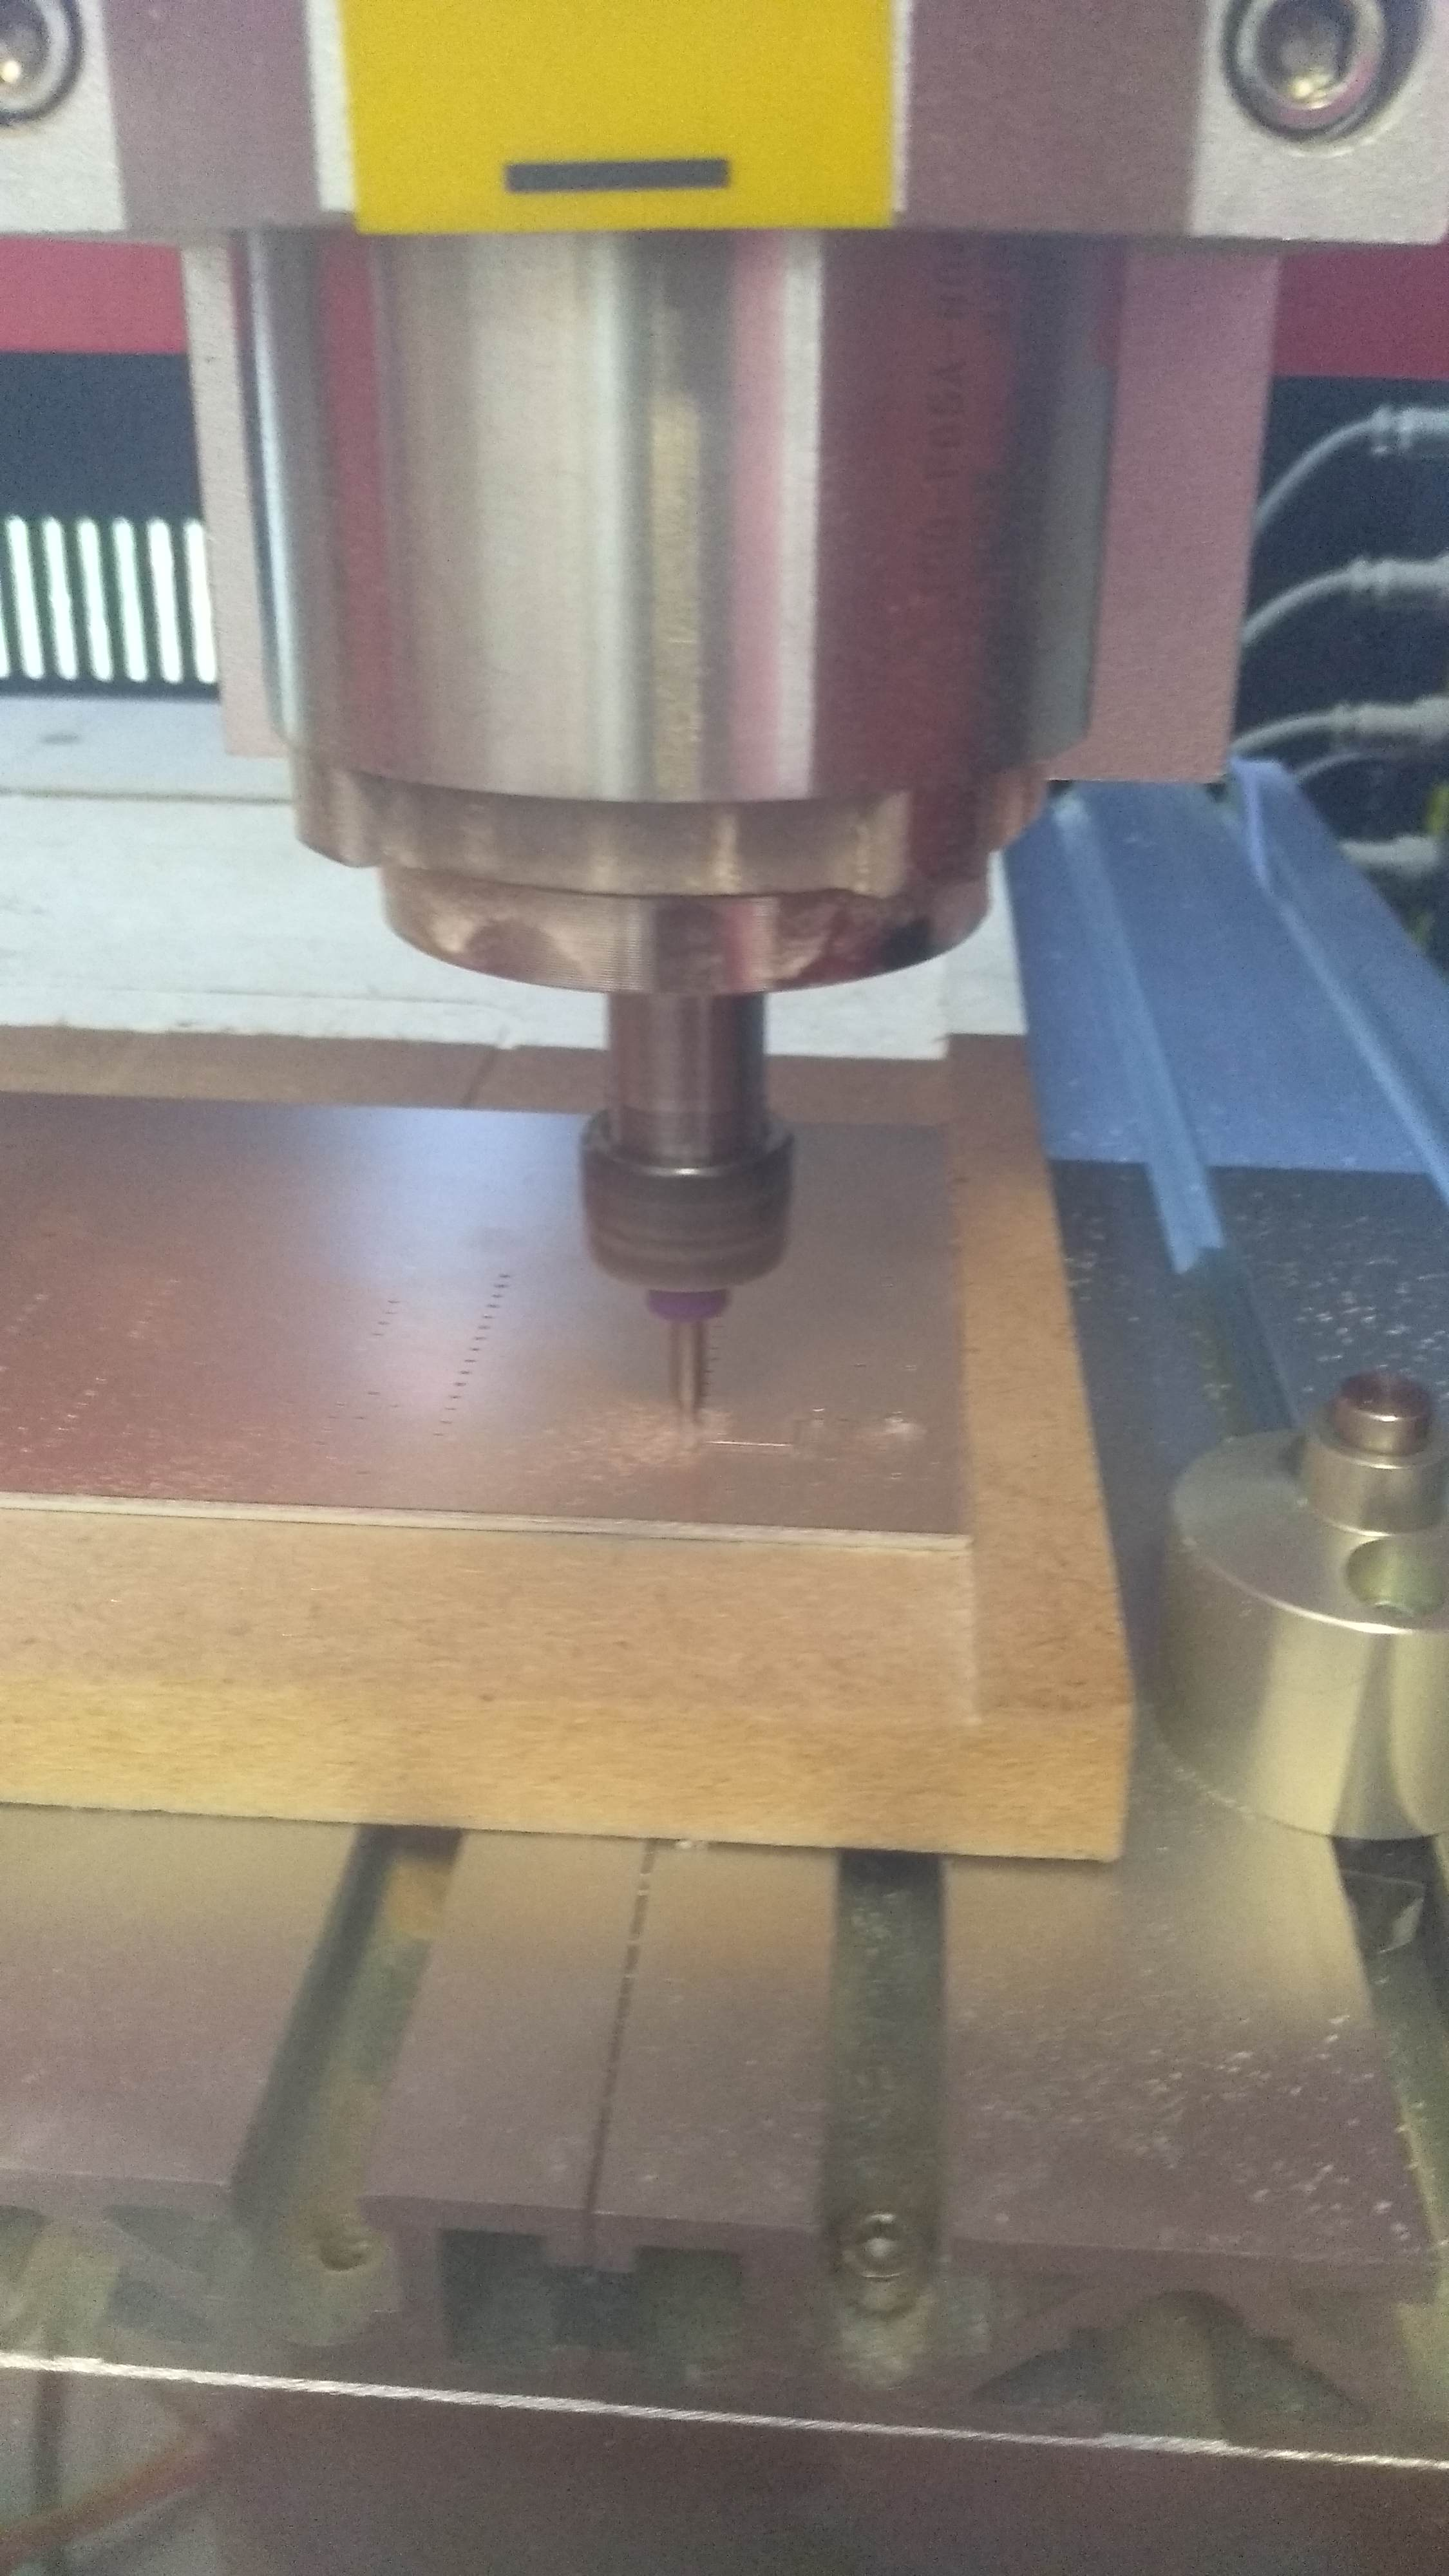
\includegraphics[width=0.2\textwidth]{img/CNCRouter.jpg}
	\label{img:RouterCNC}}
	\caption{Fabrication chez FabLab}
	\label{img:CampusFab}
\end{figure}

% \begin{figure}[!htb]
% \centering
% 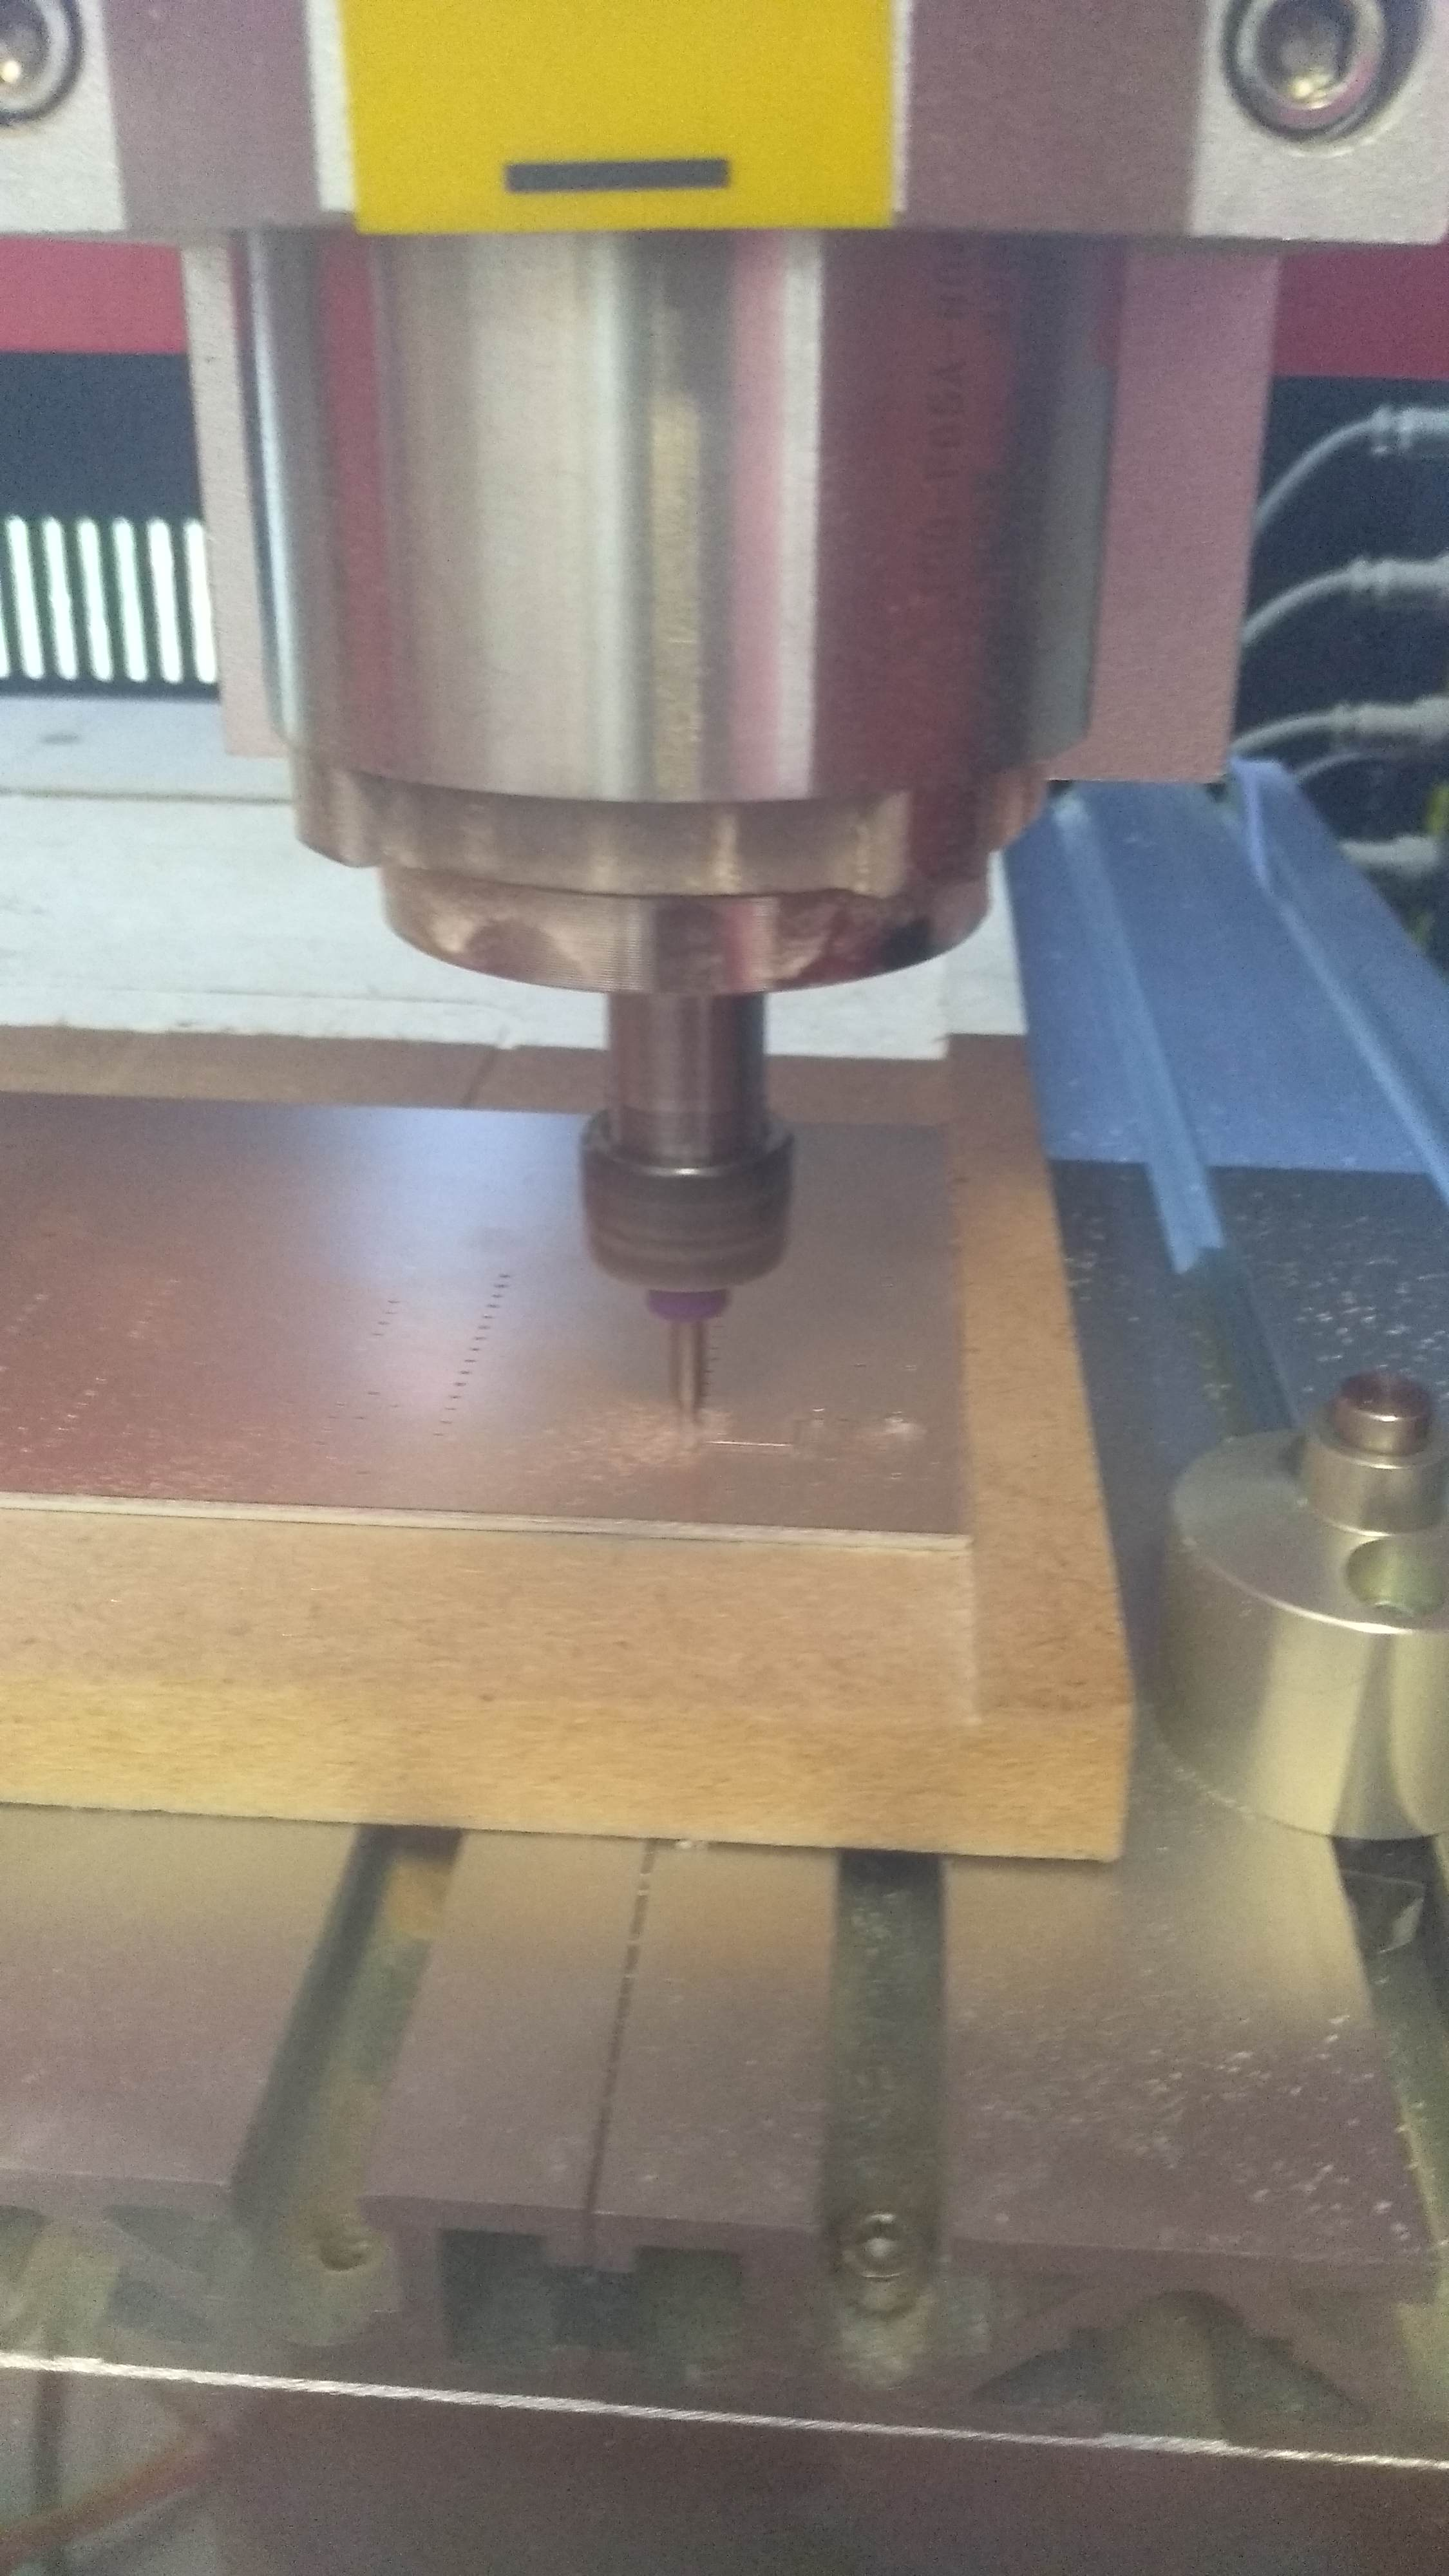
\includegraphics[width=0.2\textwidth]{img/CNCRouter.jpg}
% \caption{Machine CNC pour le routage des PCB}
% \label{img:RouterCNC}
% \end{figure}

% \begin{figure}[!htb]
% \centering
% \includegraphics[width=0.2\textwidth]{img/FlatCAM.png}
% \caption{Logiciel pour le routage des PCB}
% \label{img:flatcam}
% \end{figure}

% Luego de hacer los circuitos utilice la estacion de soldadura para montarlos componentes en la pcb.
\begin{par}
	Après avoir fabriqué les PCB j'ai soudé les composants pour monter le
	circuit.
\end{par}

\begin{figure}[!htb]
\centering
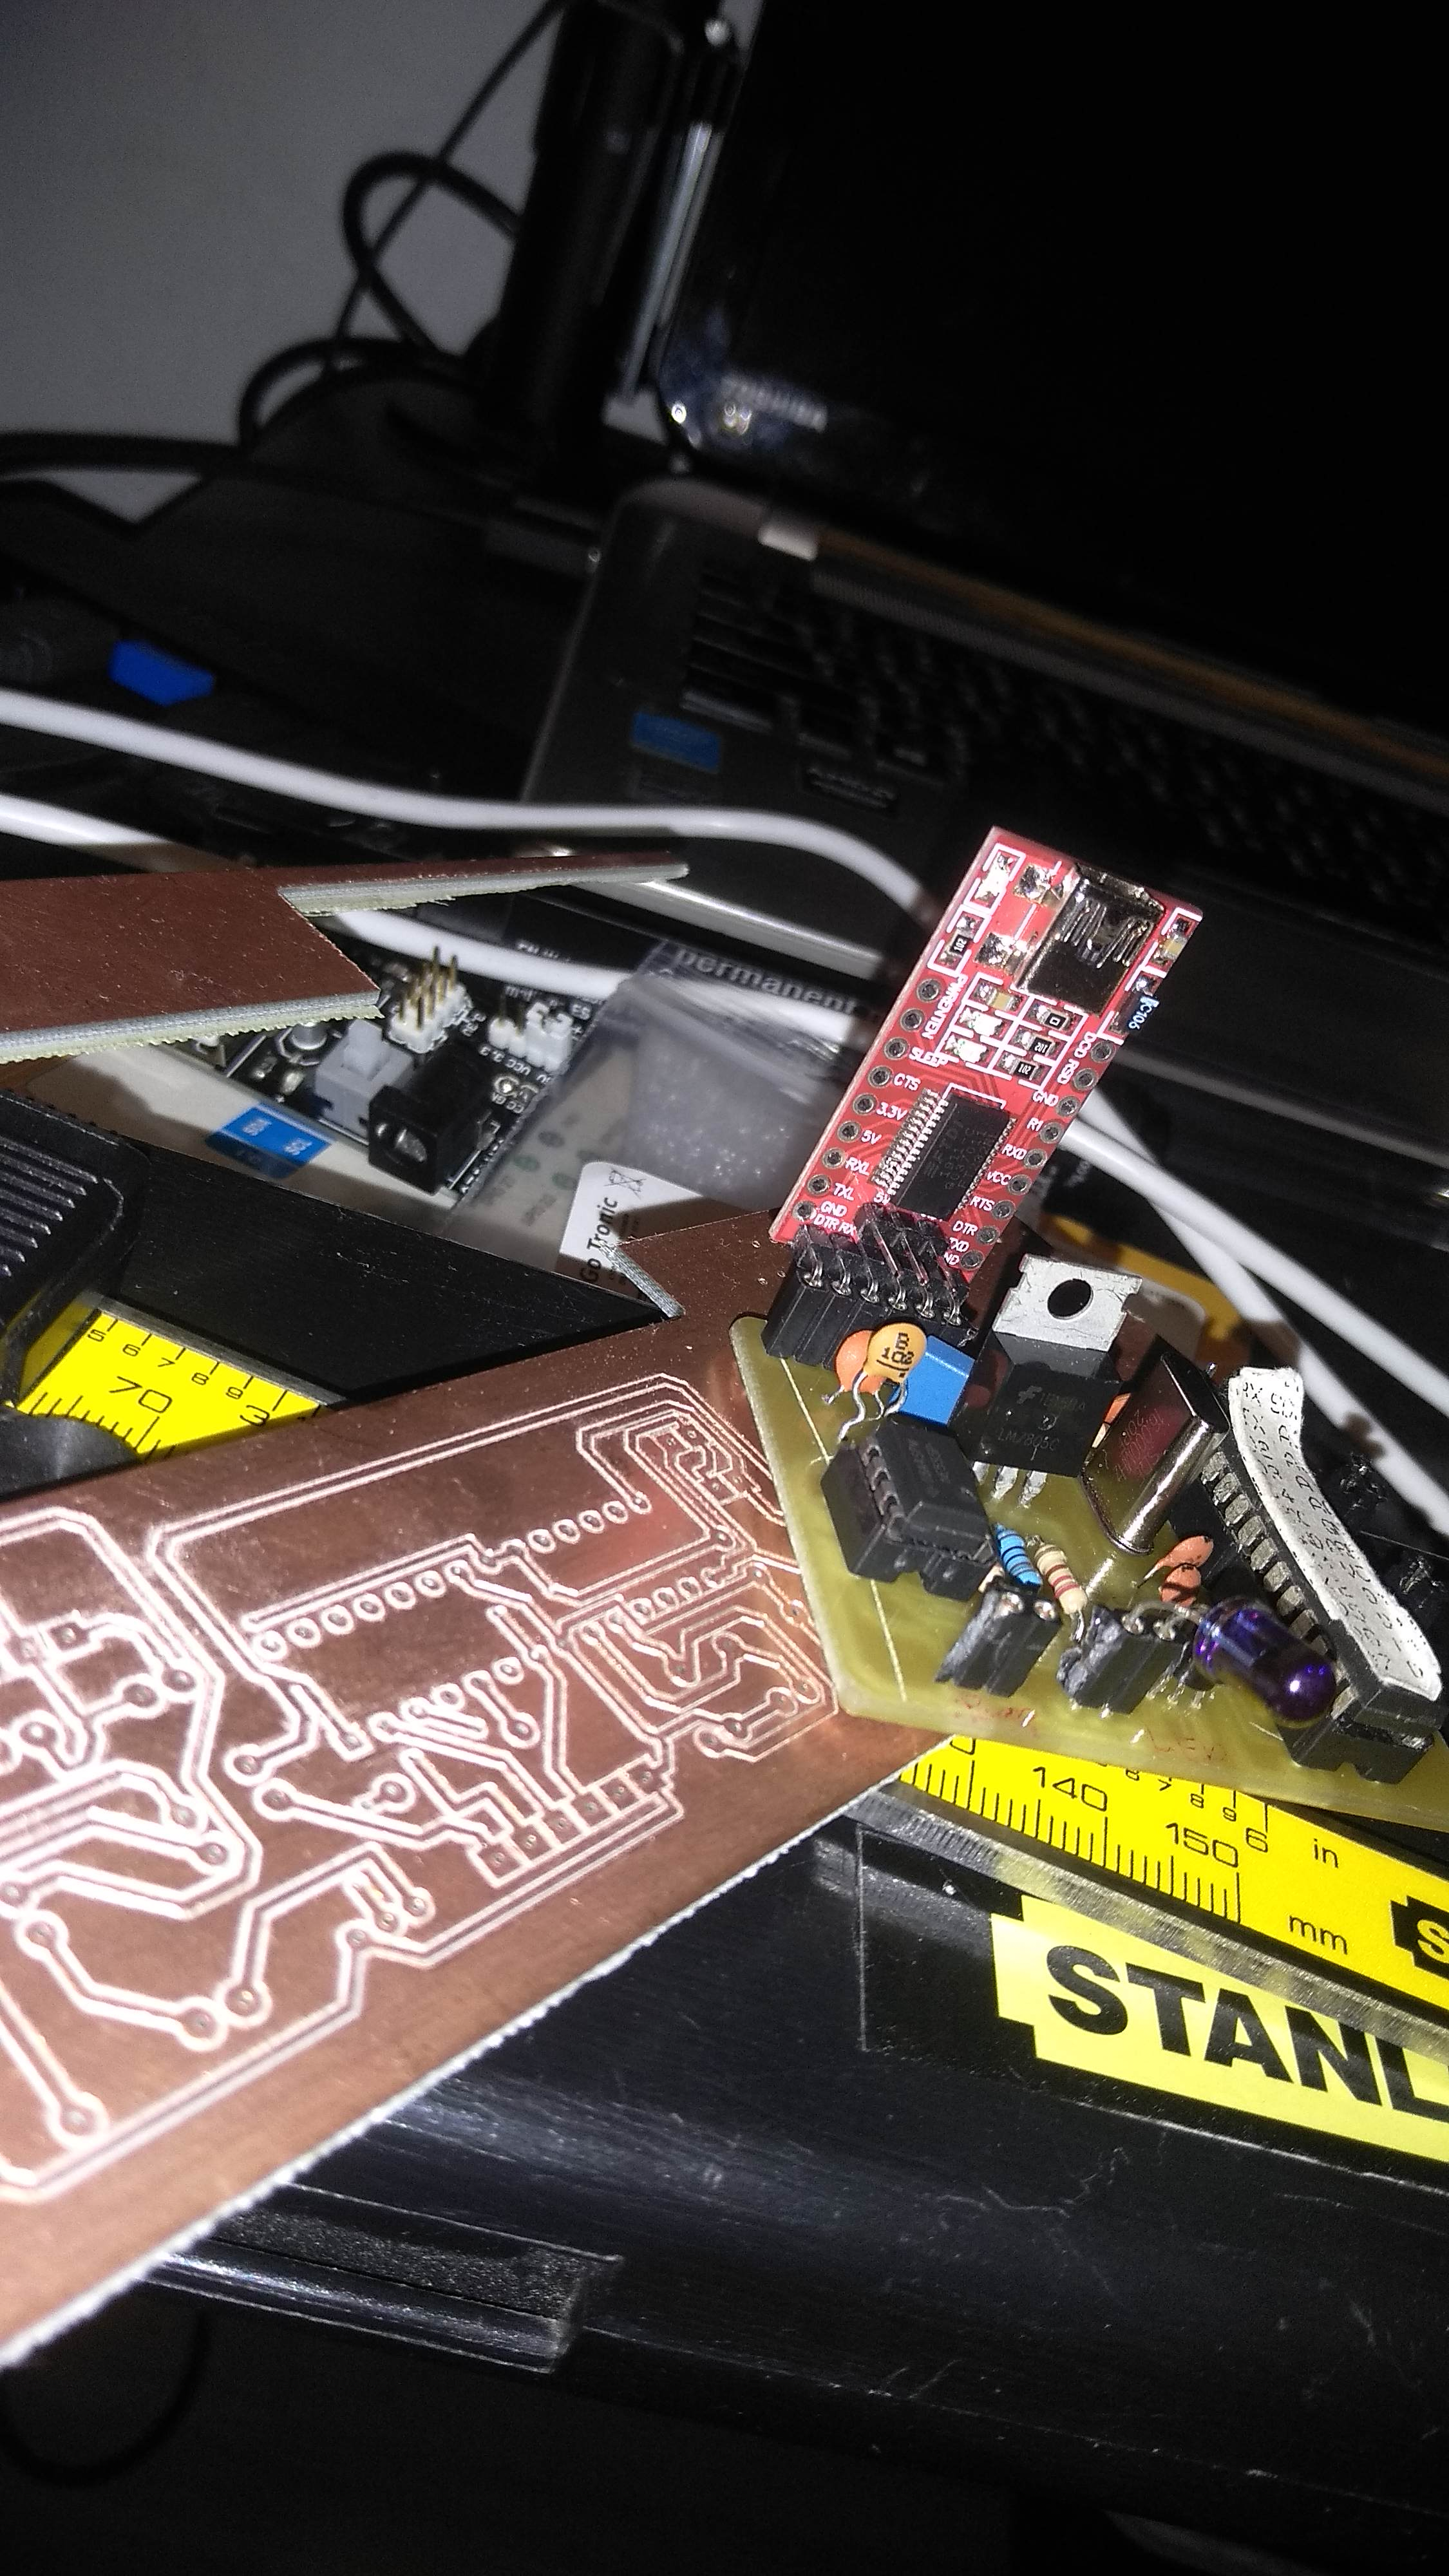
\includegraphics[width=0.2\textwidth]{img/CircuitosCNCed.jpg}
\caption{Des circuits après le CNC Router}
\label{img:CircuitsCNCd}
\end{figure}
% La ultima herramienta que utilise fue la cortadora laser para hacer el soporte de las barieres IR y la nueva cajita del starting block (mas pequenha y tales)
Un autre outil que j'ai utilisé c'était la découpe laser pour découper du plexiglas. Dans l'image \ref{img:barriere} on peut le voir.


\begin{figure}[!htb]
	\centering
	\subfigure[Découpe Laser]{\includegraphics [height=2in]{img/CortadoraLaser.png}}
	\subfigure[Premiere essaye du Barriere IR]{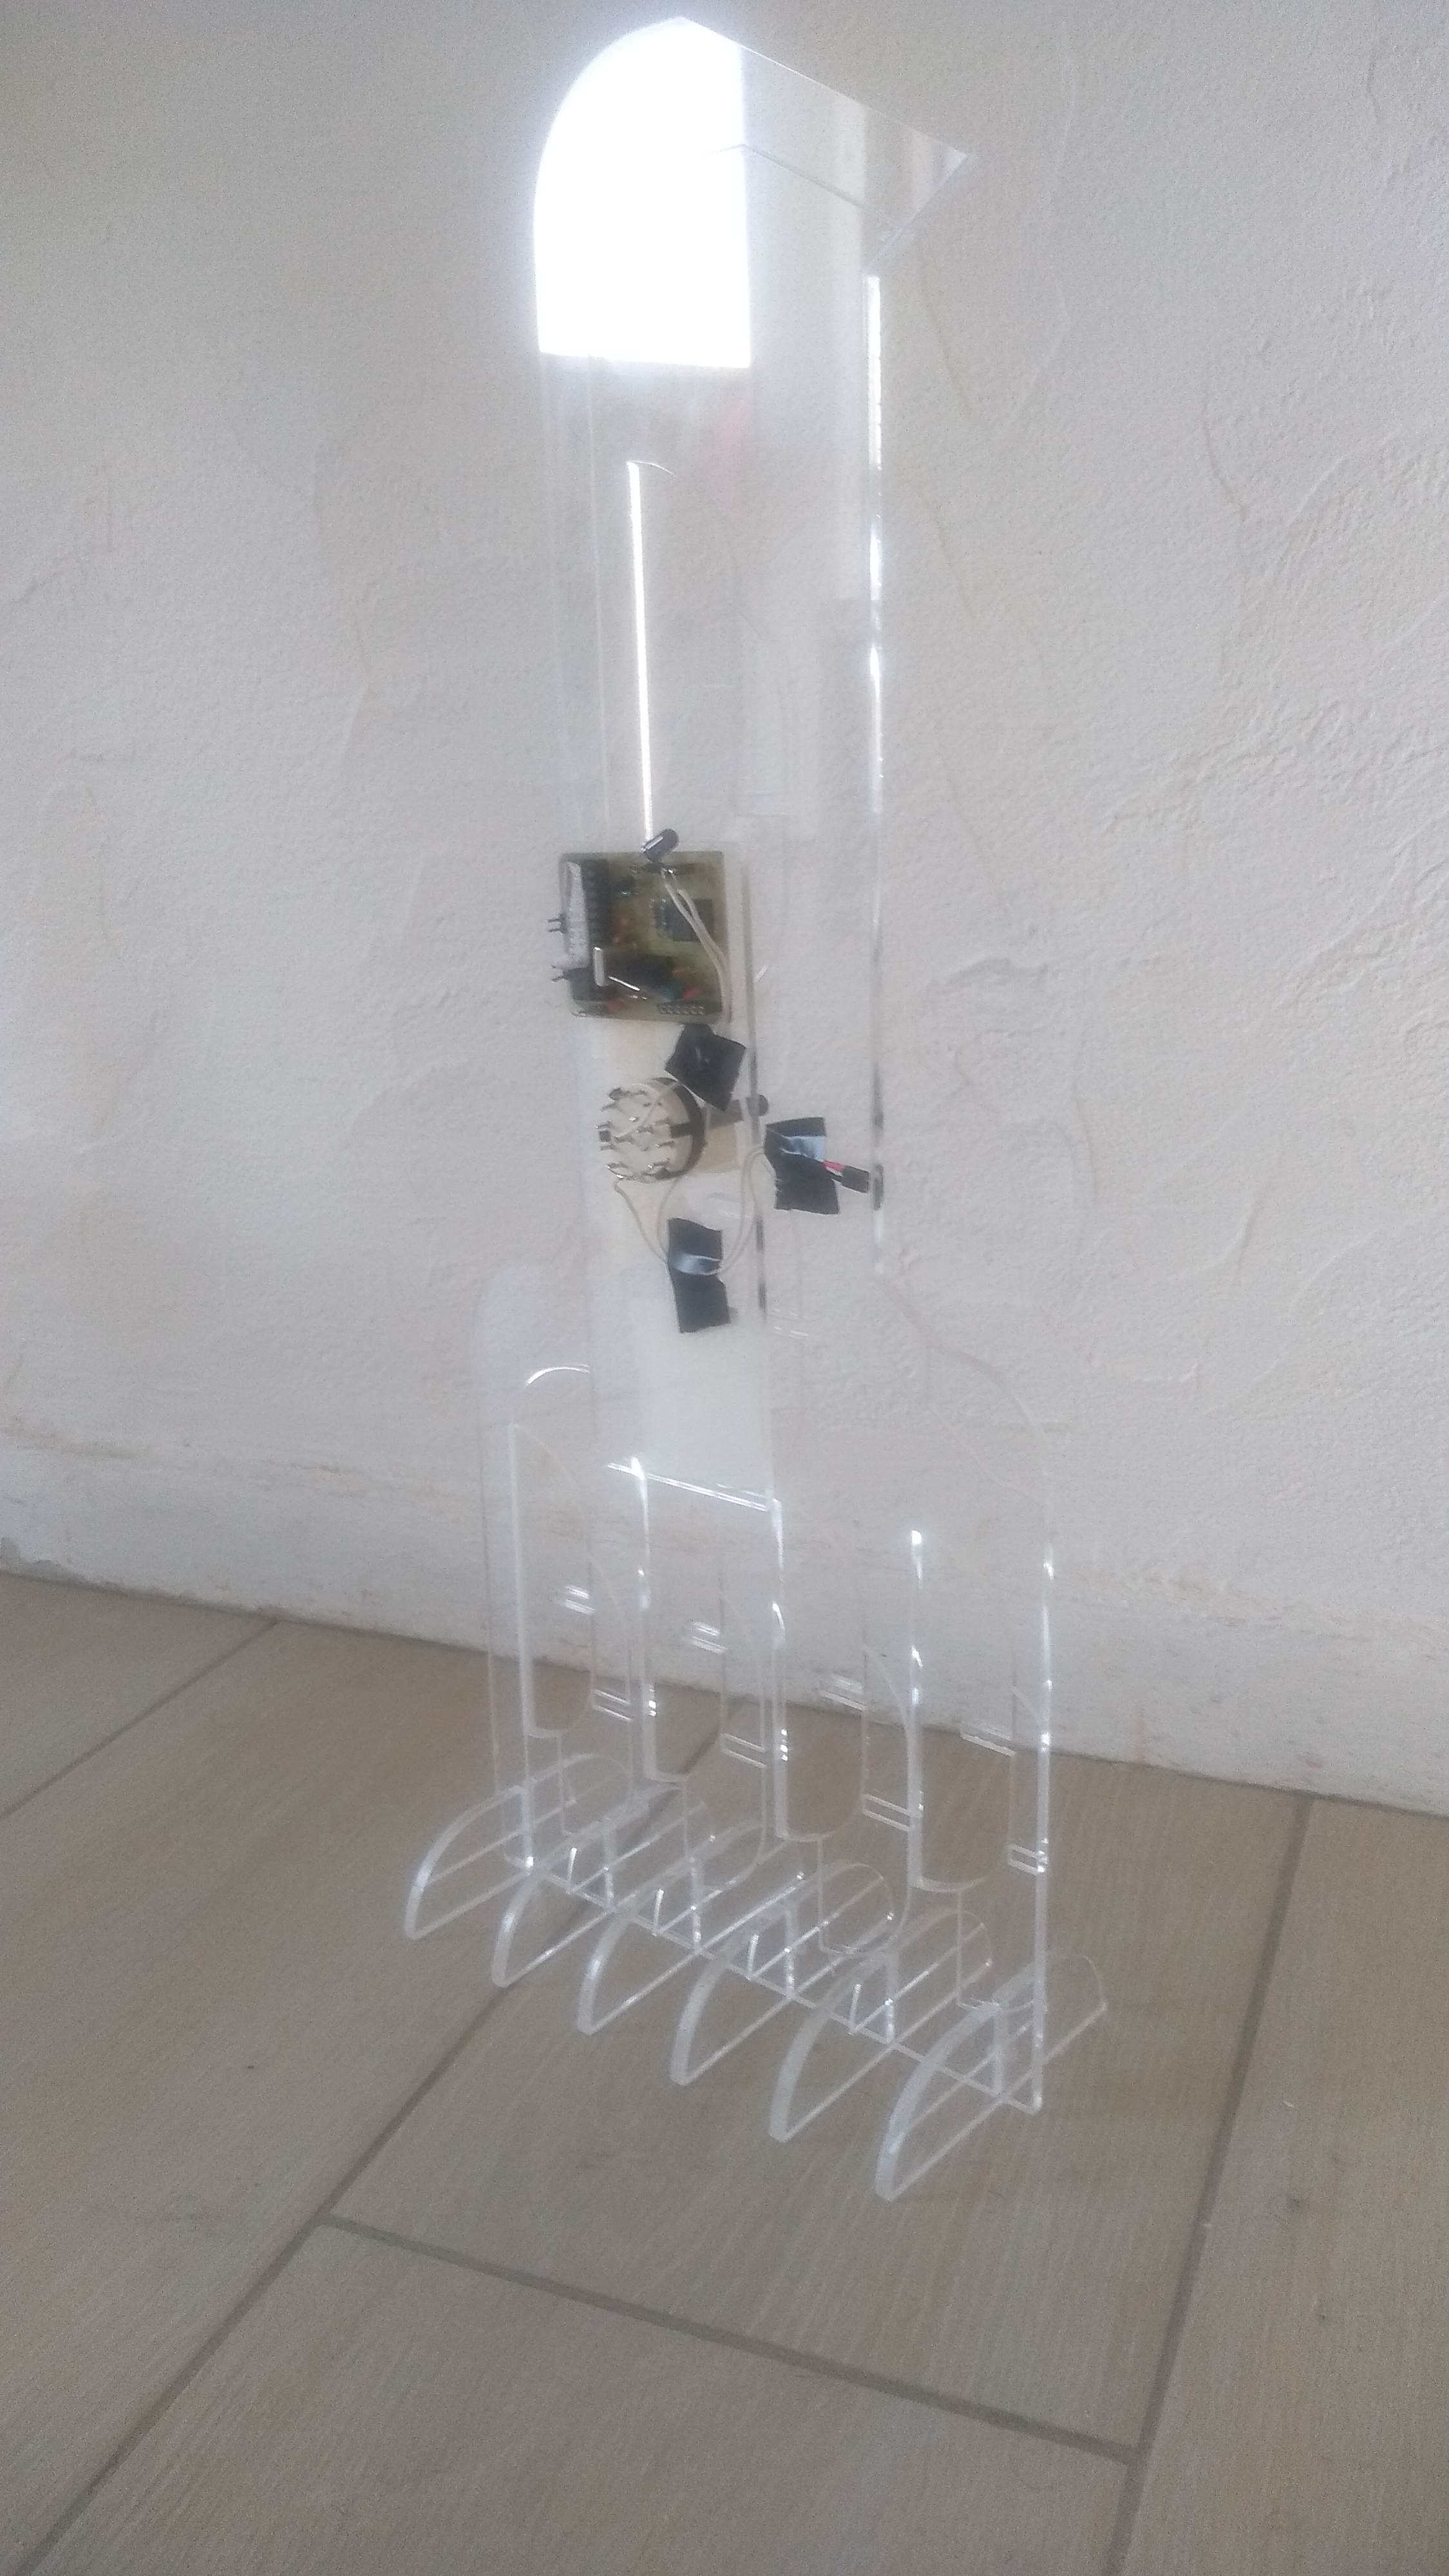
\includegraphics [height=2in]{img/BarriereIrV1.jpg}}
	\caption{Résultats de la découpe laser}
	\label{img:barriere}
\end{figure}
% La impresora 3D tenia pensado usarla para hacer el témoin en PLA transparente y estuve imprimiento un cable chain para mejorar la robustez de los cables en el starting block.

% \begin{par}
% 	J'ai failli utiliser l'imprimante 3D pour faire 
% 	quelques pièces en fin du stage mais j'ai chopé
% 	le covid les dernieres semaines du juillet.
% \end{par}

\subsection{Github}
\begin{par}
Ce projet était un projet avec une grande quantité de programmation et j'ai choisi git comme outil de gestion de versions. En plus, 	j'ai fait un repositoire sur Github pour avoir tout bien organisé et centralisé sur une seul endroit.
\end{par}
% Al ser un proyecto donde mas de la mitad del trabajo es programacion es necesario tener un gestor de versiones para el cual utilise git. Ademas Github es excelente como herramienta de gestion compartida.

% Otra ventaja de github es que ofrece una pagina de wikis donde se puede dejar toda la documentacion por si alguien retoma el proyecto donde yo lo estoy dejando ahora mismo. Tambien tiene la seccion de gestion de proyectos que es parecida a slack donde pongo lo que voy haciendo poco a poco y el tutor de stage puede revisar mi trabajo poco a poco. 
\begin{par}
 Github nous offre une page de wikis pour la documentation du projet. Dans cette section j'ai pensé laisser toutes les instructions pour les développeurs et utilisateurs en général.
\end{par}
\begin{par}
	Sur Github nous trouverons aussi une section pour gérer des projets partagés du type slack ou 	trello. Sur l'image \ref{img:git_all} on peut le voir.
\end{par}

% La seccion de issues tambien es buenisima para el trabajo en grupo y si alguien a futuro tiene problemas con mi proyecto yo puedo ayudarlo a solucionar el problema.
\begin{par}
La section issue de github permet de partager les problèmes avec autres développeurs, même si je ne fais plus partie du projet.
\end{par}

\begin{figure}[!htb]
	\centering
	\subfigure[Repositoire sur github]{\includegraphics [height=2in]{img/Repo.png}
	\label{img:git:repo}}
	\subfigure[Outil de gestion de projets de github]{\includegraphics [height=2in]{img/GithubProject.png}
	\label{img:git:project}}
	\subfigure[Wikis sur github]{\includegraphics [width=2.7in]{img/GitWiki2.png}
	\label{img:git:wiki}}
	\caption{Images du repo}
	\label{img:git_all}
\end{figure}

%-------------------------- * Seccion de resultados * --------------------------------

\section{Results}
% Los resultados se vieron afectados por varios factores ajenos al desarrollo del proyecto como mi rattrapage a mitad de junio, varias pcb que vinieron malas y faltando dos semanas para terminar el stage me dio covid y cuando pude salir el fablab estaba cerrado y solo me faltaba terminar de fabricar las piezas del temoin. Para colmo se quemaron 2 step up y no pude nisiquiera pude soldar los temoin (y habia uno que tenia unos vias que no hacian conexion, maldita sea). A pesar de todo eso pude avanzar mucho en otras cosas.
\begin{par}
Le projet a eu un développement lent dû à ma manque d'expérience mais en général j'ai bien géré les temps. Quand même, j'ai eu des problèmes à cause des cartes électroniques défectueuses.
\end{par}
\begin{par}
Pour la partie software, j'avais déjà travaillé avec python et le framework de l'interface ce qui m'a rendu un peu facile le travail de programmation.
\end{par}
\begin{par}
Comme dernier souci j'ai eu le covid en fin du stage et je n'ai pas pu finir la fabrication de quelques composants chez CampusFab parce que j'ai dû me confiner. Ces jours de confinement j'ai avancé la programmation d'une base de données plus robuste et prête à utiliser même sans les prototypes.
\end{par}

%-------------------

\subsection{Dock multiplateforme}
% La raspberry como dock multifuncional es le mejor avance que hice ya que ahora tiene una base de datos que permite ingresar atletas, coachs y llevar un historal de todas las sesiones de entrenamiento. Ademas se conecta directamente al starting block y permite ver su estado de bateria. 
% Tambien permite actualizar la interfaz directamente desde github, lo que permitiria venderlo como producto y actualizarlo con el pasar del tiempo.
% Toda la informacion guardada es ademas exportable por si se quiere hacer un tratamiento de datos externo.

\begin{par}
	Le dock multi plateforme est 	l'avancement le plus remarquable de mon stage. Il 	a une base de données complète avec l'information 	de chaque coach et athlète. Sur l'image \ref{img:gui_all} 	on peut voir la liste de séances et le graph généré 	par le dock.
	Il se connecte avec 	un smartphone, tablette ou même un ordinateur via 	Wi-Fi direct pour manipuler et voir les données.	Sur l'image \ref{img:gui:landing-page} on peut voir 	la première page de l'interface vue depuis un 	ordinateur.
\end{par}

\begin{figure}[!htb]
	\centering
	\includegraphics[width=0.4\textwidth]{img/LandingPage.png}
	\caption{Page d'accueil}
	\label{img:gui:landing-page}
\end{figure}

\begin{figure}[!htb]
	\centering
	\subfigure[Seance Detaillé]{\includegraphics [height=2in]{img/SessionDetail}
	\label{img:gui:session-detail}}
	\subfigure[Liste de seances stockées]{\includegraphics [height=2in]{img/SessionList}
	\label{img:gui:session-list}}
	\caption{Base de données.}
	\label{img:gui_all}
\end{figure}

% \begin{par}
% 	En plus, elle peut \^etre mise à jour avec github
% 	et donc si on change des choses sur l'interface au 
% 	niveau du graphisme ou de manipulation de donées
% 	de l'autre c\^oté du monde, on peut voir ces 
% 	changements sur la raspi.
% \end{par}
\begin{par}
	Malheureusement la partie de hardware pour connecter 	les témoins et extraire les données n'a pas pu être 	finie à cause du covid parce que je n'ai pas pu aller 	chez CampusFab pour finir la fabrication.
	% lastimosamente la parte de los temoins no la pude
	% terminar por el covid y porque la mayoria de las 
	% tarjetas electronicas del servicio de la fac vinieron
	% con defectos.
\end{par}

\subsection*{Travail à futur}
% Como mejora esta meterle una bateria y que esta cargue los temoins. Mostrar tambien la carga del propio aparato. y terminar la parte que se conecta con el temoin, la cual esta testeada con datos simulados que funcionan bien.
% Otra mejora que tengo pensado ponerle es una opcion que permita un calibrage automatico de los sensores de fuerza para no tener que desarmar el dispositivo cada vez que se descalibre.
\begin{par}
	La première chose à améliorer est avoir une batterie qui charge 	les témoins et qui donne une bonne autonomie au dock et finir la 	partie de connexion pour les témoins.
	% Meterle una bateria para que cargue los temoins, hacerle la conexion para que se connecte con los temoins y 
	% de paso que los cargue. Hacerle pruebas para calcular la autonomia de la bateria y la vaina.
\end{par}
% \begin{par}

% 	Algo que me gustaria agregarle es una parte de calibrage automatico de los sensores de presion
% 	en el starting block
% \end{par}

%-------------------

\subsection{Startingblock 2.0}
% El mayo cambio en el starting block en terminos de harwdware es su tamanho mas reducido y el uso de una bateria de ion de litio recargable directamente desde la cajita. Segun las pruebas de rendimiento el dispositivo consume aproximadamente unos 100mA de corriente de forma constante con pequenhos picos de corriente de 200mA por lo cual se puede estimar la duracion de la bateria. (aqui pones fotos del videito que grabaste)
\begin{par}
 	La boîte électronique du starting bloc est plus 	petite et plus efficace d'un point de vue énergétique.	Maintenant il a un chargeur interne avec une connexion 	mirco-usb qui permet de le charger avec un chargeur commercial. Image \ref{img:sb:complete}
\end{par}

\begin{figure}[!htb]
	\centering
	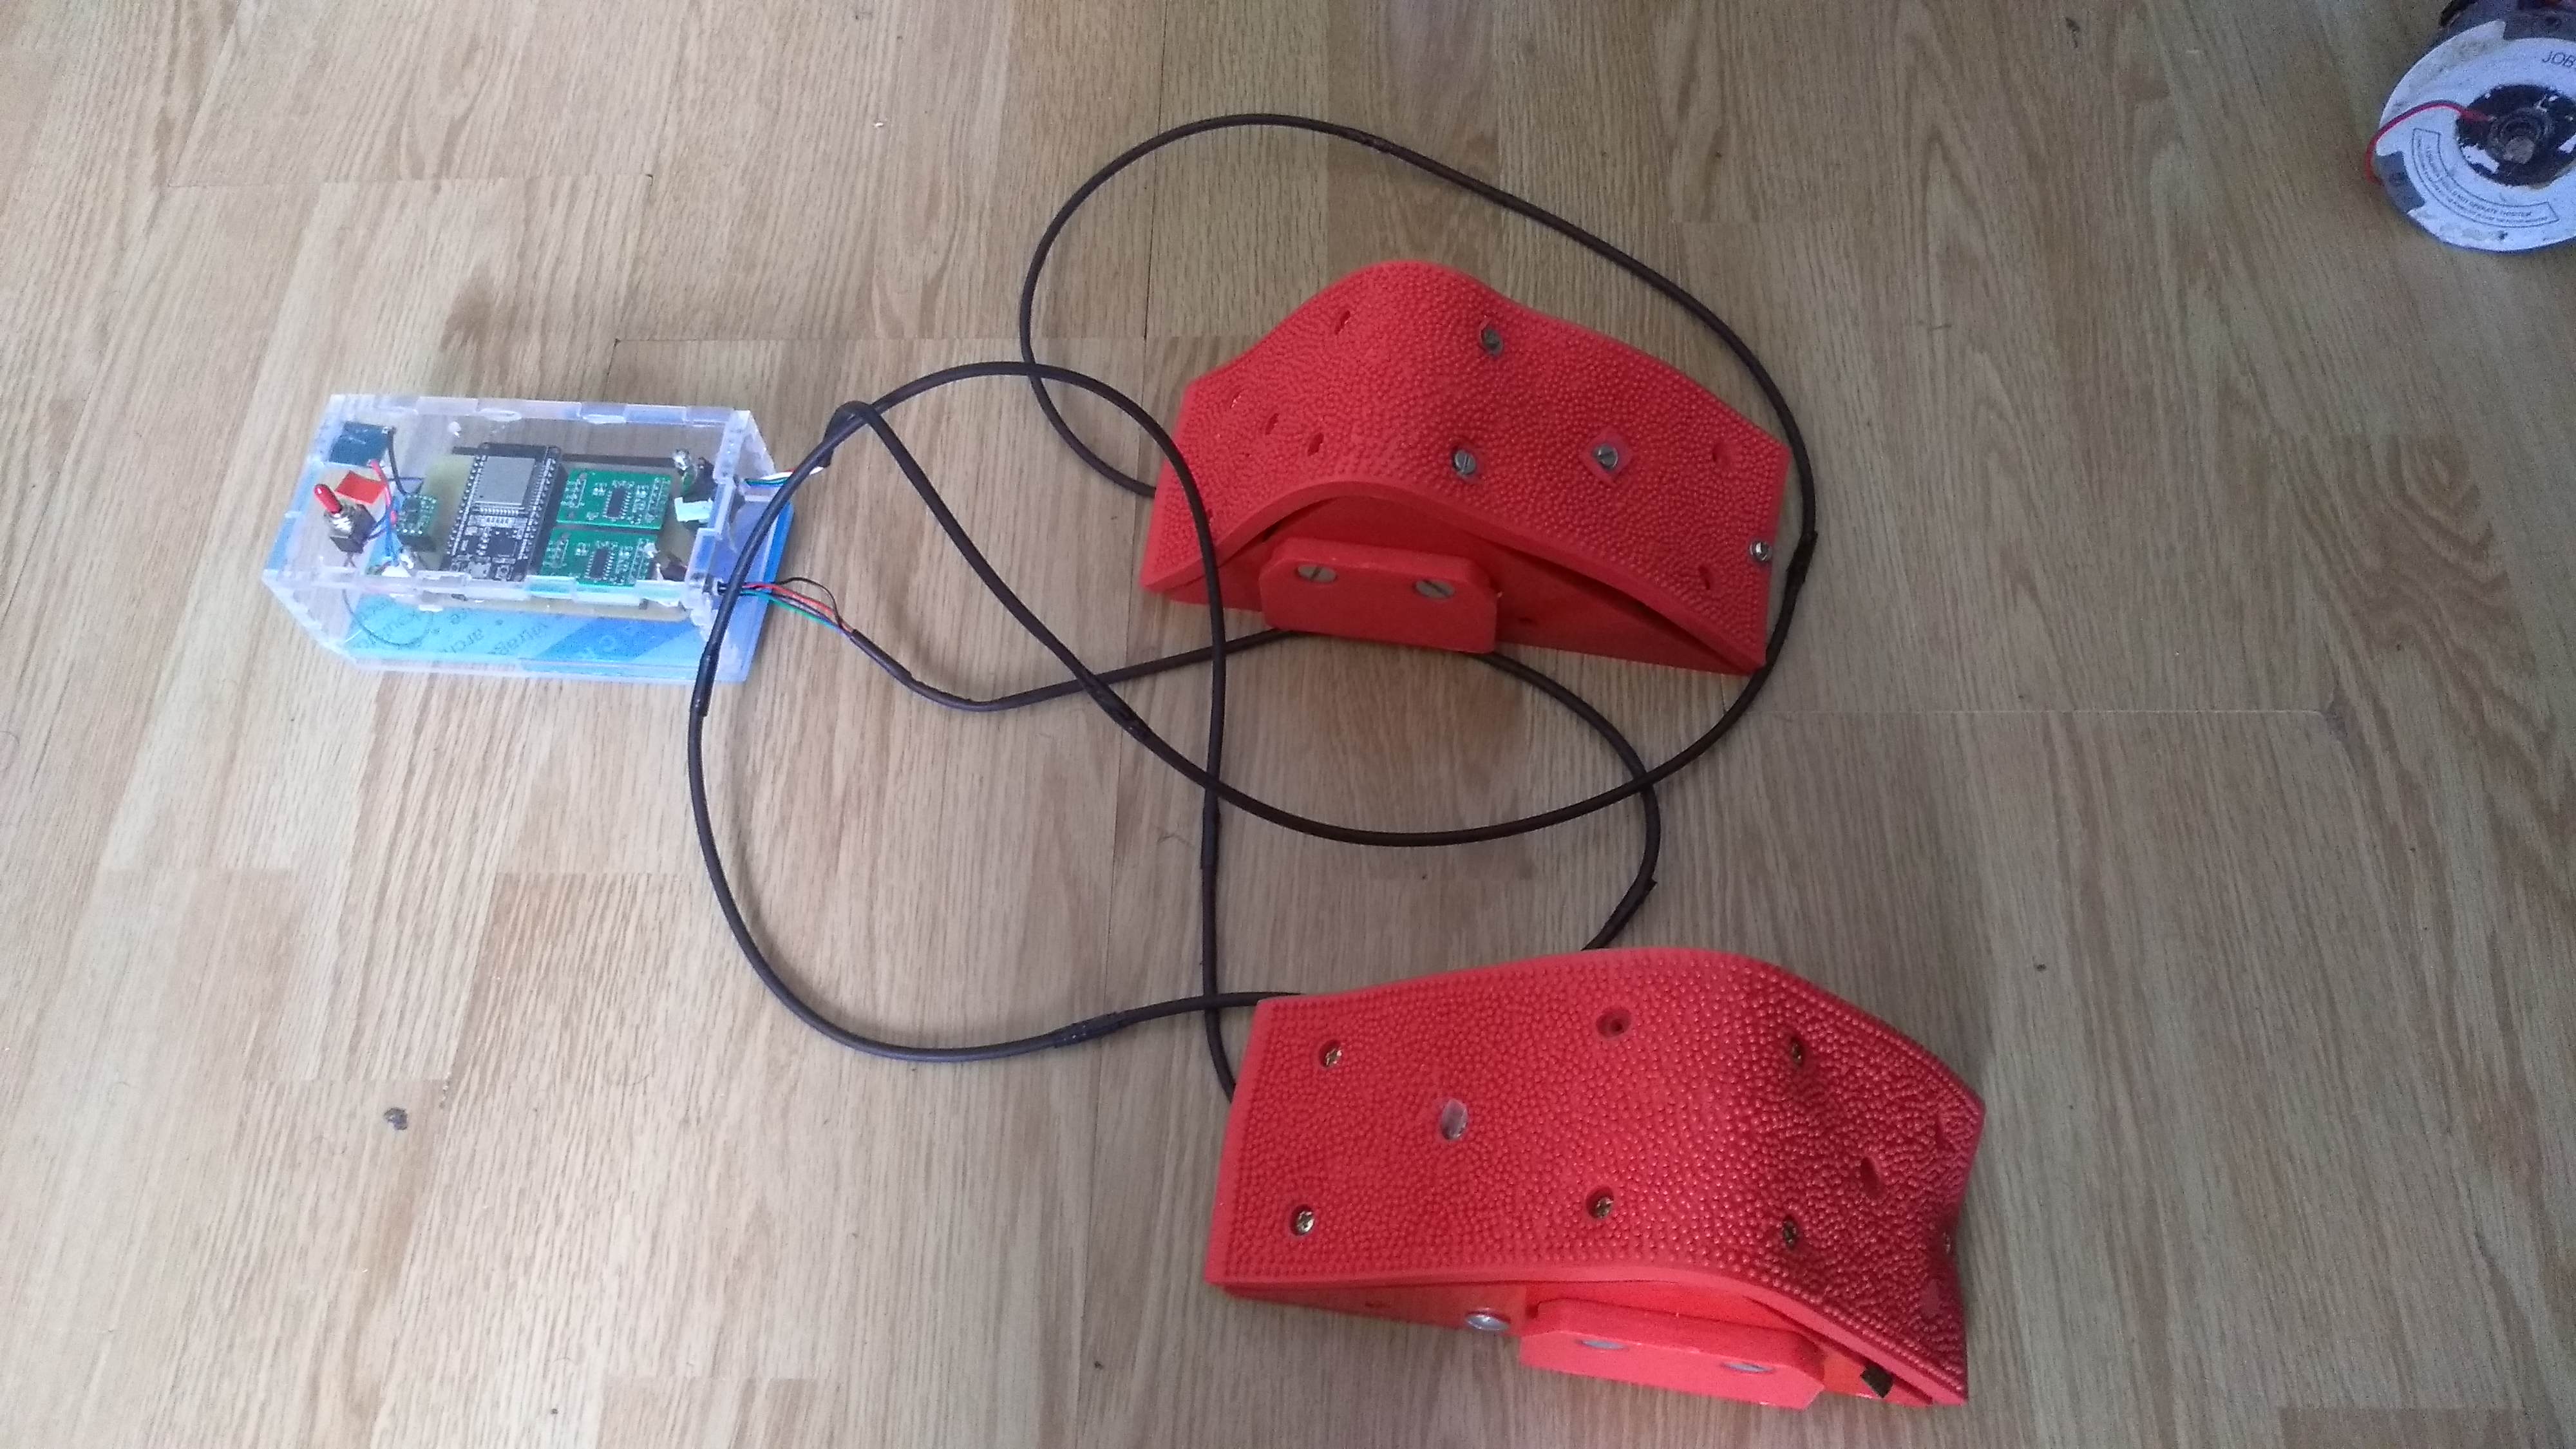
\includegraphics[width=0.5\textwidth]{img/StartingBlockCompleto.jpg}
	\caption{Starting Block}
	\label{img:sb:complete}
\end{figure}

\subsection*{Travail Futur}
\begin{par}
	Ajouter un script de calibration lancé par le dock. 	Améliorer la conception pour un possible dépannage et 	un condensateur qui aide 	la batterie dans les piques de courant.
\end{par}
% Agregarle a la programacion el programa de calibracion (el cual ya viene listo en la libreria de los amplificadores) que se haga directamente desde la interfaz grafica.

% Otra cosa que no tuve en cuenta es el disenho que favorezca un depanage. Actualmente es muy complicado desarmar todo para revisar si algo falla, eso fue un error de disenho que no tuve en cuenta.
% Una ultima mejora es agregarle un capacitor que ayude a la bateria en los picos de corriente para aumentar la vida util de la bateria.

%-------------------

\subsection{Témoin et Course de relais}
% Los temoin y las barrieres IR tuvieron una mejora sustancial en terminos de usabilidad y componentes. Lastima que las pcb del protipo final vinieron con fallas y no se pudo armar un dispositivo final, ademas que habian unos step up que se quemaron y solo me quedaba uno y lo use para el starting block que ya estaba armado para tener una cosa que sirviera. Ademas de todo esto, la imposibilidad de ir al fablab la ultima semana me limito mucho porque tuve covid y aja eso me cago la vida.
\begin{par}
	Les témoins et les barrières IR ont eu une upgrade 	énorme avec les nouveaux composants. Fâcheusement 	les cartes électroniques faites par l'université 	avaient des défauts de fabrication et quelques 	composants de puissance ont brûlé lorsque le service de commandes de l'université est allé en congé.
\end{par}
\subsection*{Travail Futur}
\begin{par}
 Il me manque monter et tester les prototypes, mais j'ai déjà pensé à faire une conception un peu plus adaptée au dépannage rapide.
\end{par}
% Basicamente falta armarlos y probarlos, ahi falle pero me perjudico la situacion sanitaria ya que esta semana tenia pensado hacer esas cosas.

%-------------------

\subsection{Documentation du projet}

\begin{par}
	La documentation du projet se trouve sur la page de wikis du repo
	sur github. Elle a des sections pour les futurs developeurs et pour
	les futurs utilisateurs.
\end{par}
\begin{par}
	Pour la documentation des codes en C et C++ j'ai utilisé d'Oxygen.
\end{par}
% La documentacion actual es la de la version del poryecto TER y me falta agregarle todas las cosas que desarrolle hasta este momento. Viendo que utilise un framework web y que no todo el mundo sera capaz de utilizar este framework intente factorizar las funciones al maximo para que cualquier pueda modificar las funciones que hacen las cosas importantes sin tener que meterse directamente con el framework.
% Para documentar tambien utilise doxygen que genero un archivo pdf con la explicacion de todas las funciones en C.

\begin{figure}[!htb]
	\centering
	\includegraphics[width=0.5\textwidth]{img/GitWiki.png}
	\caption{Wikis du Github}
	\label{img:git:wikis1}
\end{figure}

\subsection*{Travail Futur}
\begin{par}
 Vu que j'utilise Django, un framework optimisé pour le web, j'aimerais documenter le fonctionnement du framework pour les développeurs qui ne sont pas habitués à ce type de fonctionnement.
\end{par}
% Me encantaria documentar todo el framework de django pero es un trabajo largo y duro, asi que lo dejo como trabajo futuro.

%\begin{figure}[!htb]
%\centering
%\includegraphics[width=0.2\textwidth]{images/ubication-sipi.png}
%\caption{Location du village Sipí \cite{sipi:ubicacion}}
%\label{img:sipi:ubicacion}
%\end{figure}

% Plantilla para colocar muchas imagenes con un multiplot
%\begin{figure}[!htb]
%\centering
%\subfigure[Photo trouvé sur Facebook]{\includegraphics %[height=2in]{images/image18.png}
%\label{img:sipi-urbana}}
%\subfigure[Photo prise par la mairie de Sip\'i ]{\includegraphics %[height=2in]{images/alcaldia-sipi.jpg}
%\label{img:sipi-urbana2}}
%\subfigure[Photo pris par le quotidien Colombien \textit{CNC Noticias}]{\includegraphics %[width=2.7in]{images/image39.png}
%\label{img:sipi-urbana3}}
%\caption{Images de Sip\'i}
%\end{figure}
%Sur la Figure \ref{img:sipi:boats} on peut voir les bateaux transportant des personnes et des biens.



%Para citar la bibliografia haces \cite{Photovoltaic}
%Para referenciar las imagenes haces lo sgte \ref{fig:schema}


\section{Conclusion}
% Este stage fue muy interesante y aprendi muchas cosas como gestionar un proyecto, usar diferentes logiciels para plantear las cosas e incluso utilise plantuml para planear las cosas pero no funciono del todo, cagada eso. Aprendi mucho y estuvo bueno todo mientras duro.
\begin{par}
 Ce stage a été très enrichissant parce que c'est la première fois que je fais un projet financé par une université, d'habitude nous avons limitation technologique en tant qu'étudiants mais dans ce projet j'ai eu un budget plus généreux et cela m'a fait rechercher les meilleurs composants pour le projet.
\end{par}
\begin{par}
	% C'etait interesant aussi faire la conception,
	% fabrication et montage de chaque un des appareils
	% du projet.
 J'ai bien aimé faire partie de la conception, fabrication et montage de chaque appareil.
\end{par}
\begin{par}
	Je veux suivre ce projet en tant que stagiaire pour 	l'année prochaine et faire une alternance (si possible) 	pour faire toutes les améliorations proposées précédemment.
\end{par}

%debes hacer esto para meter archivos de otro lado
%\input{sub_files/Calcul_puissance}
%\label{anexe:calcul-puissance}
%-------------------

%Para meter un pdf haces lo sgte 
%\includepdf{images/Velocidad-Maxima-Energia_13}
%\label{pdf:vent_vitesse_max}
%-------------------

% \begin{figure}
%     \centering
%     \includegraphics[height=\textheight]{Anexes/RadiacionSolar13 (1).pdf}
%     \caption{Caption}
%     \label{fig:radiacion}
% \end{figure}


% Plantilla para colocar muchas imagenes con un multiplot
%\begin{figure}[!htb]
%\centering
%\subfigure[]{\includegraphics [width=2.5in]{lab_2_vision_15.png}}
%\subfigure[]{\includegraphics [width=2.5in]{lab_2_vision_16.png}}
%\subfigure[]{\includegraphics [width=2.5in]{lab_2_vision_17.png}}
%\caption{Paleta de colores}
%\end{figure}

% Plantilla para poner una imagen cualquiera
%\begin{figure}[!htb]
%\centering
%
%\caption{Histograma de la imagen}
%\end{figure}

%\bibliography{Biblio}

\end{document}
